\documentclass{article}

\usepackage{../template}

\usepackage{cleveref}
\usetikzlibrary{knots}

\usepackage{subfig}
% \usepackage{caption}
% \usepackage{subcaption}
%
% \DeclareCaptionFormat{subfig}{\figurename~#1#2#3}
% \DeclareCaptionSubType*{figure}
% \captionsetup[subfigure]{format=subfig,labelsep=colon,labelformat=simple}

\title{05: Wielomian Jonesa\\ węzłów alternujących}
\author{Weronika Jakimowicz}
\date{27.03.2024}

\declaretheorem[
   name=Fakt,
   numbered=no,
   style=uwagi-lematy
]{fuck}

\declaretheorem[
   name=Twierdzenie,
   numbered=no,
   style=twierdzonka
]{thm}

\renewcommand{\contentsname}{Spis sznurków}
 
\renewenvironment{proof}{{\bfseries\color{orange} Dowód}$ $\newline}{
  \begin{flushright}
\includegraphics[width=30pt]{Donald_Duck.png}\end{flushright}$ $\newline
}

\setcounter{secnumdepth}{0}

\begin{document}
\maketitle
\thispagestyle{empty}

\def\dupa{\textwidth - 4cm}
\begin{tikzpicture}[overlay, remember picture]
  \foreach \i in {0,..., 10} {
    \pgfmathparse{Mod(\i,2)==0?1:0)}
    \ifnum\pgfmathresult>0 
      \node at (4-1*\i,4.7) {
\includegraphics[width=1cm]{kaczusia.png}};
    \else 
      \node at (4-1*\i, 4.3) {
\includegraphics[width=1cm]{kaczusia.png}};
    \fi
  }
  \foreach \i in {0,..., 10} {%\node at (\dupa + \i*1cm, 4.5) {
\includegraphics[width=1cm]{kaczusia.png}};
    \pgfmathparse{Mod(\i,2)==0?1:0)}
    \ifnum\pgfmathresult>0 
      \node at (\dupa+\i*1cm,4.7) {
\includegraphics[width=1cm]{kaczusia.png}};
    \else 
      \node at (\dupa+\i*1cm, 4.3) {
\includegraphics[width=1cm]{kaczusia.png}};
    \fi
  }
\end{tikzpicture}


\tableofcontents\setcounter{page}{0}
\newpage 
\pagestyle{plain}

\subsection{Definicja węzła alternującego}

Mówimy, że diagram regularny $D$ węzła $K$ jest alternujący, jeśli poruszając dowolny punkt $P\in D$ wzdłuż $D$, ciągle w jedną stronę, będziemy na zmianę pokonywać skrzyżowania górą i dołem.

\begin{deff}[węzeł alternujący]
  Węzeł $K$ jest alternujący, jeśli posiada przynajmniej jeden diagram alternujący.
\end{deff}

Najprostszy (o najmniejszej liczbie skrzyżowań) węzeł niealternujący to np. $8_{19}$ (ale też $8_{20}$ i $8_{21}$), który widać na \cref{diagram 8 19}. Do pokazania, że naprawdę nie kłamię jeśli chodzi o jego niealternującą naturę, wrócimy przy okazji powierzchni Seiferta i \emph{sygnatury węzła}.
\begin{figure}[h]\centering
  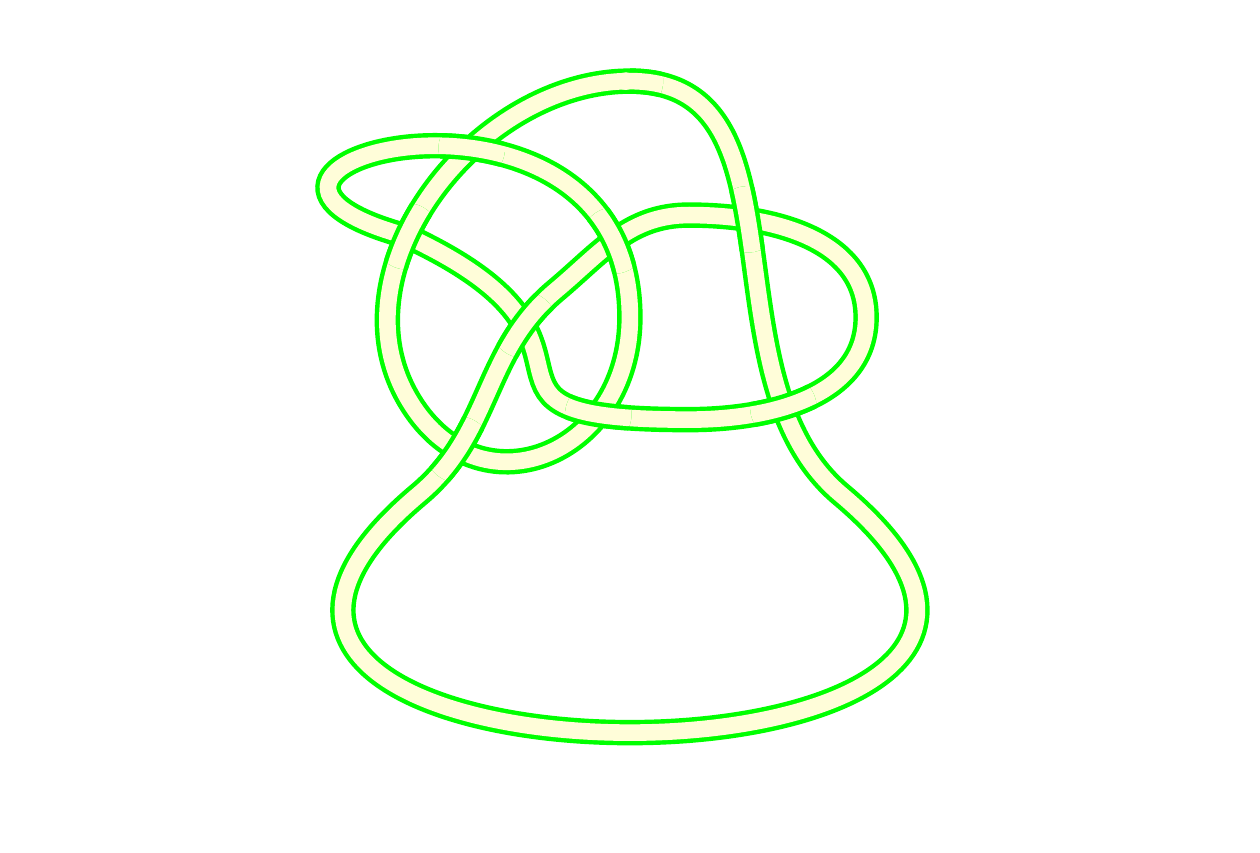
\begin{tikzpicture}
    \coordinate (a0) at (0,0);
    \coordinate (a1) at (90:3);
    \coordinate (a2) at (-40:3.5);
    \coordinate (a3) at (220:3.5);
    \coordinate (a4) at (160:1);
    \coordinate (a5) at (60:1.5);
    \coordinate (a6) at (0:3);
    \coordinate (a7) at (-60:1.5);
    \coordinate (a8) at (160:3);
    \coordinate (a9) at (200:3);

    %\foreach \i in {0,...,9} \fill (a\i) circle (3pt);
      
    \begin{knot}[
      clip width=2,
%      draft mode=crossings,
      consider self intersections,
      ignore endpoint intersections=false,
      flip crossing=2,
      flip crossing=6,
      flip crossing=8,
      line join=round,
      background color=white,
        only when rendering/.style={
        draw=green,
        ultra thick,
        double=yellow!15,
        double distance=6pt,
        %line cap=round,
      }
      ]
        \strand[thick] 
        (a1) to[out=0, in=140]
        (a2) to [out= -40, in=-140, looseness=3]
        (a3) to [out=40, in=-140]
        (a4) to [out=40, in=180]
        (a5) to [out=0, in=90]
        (a6) to [out=-90, in=0]
        (a7) to [out=180, in=-25, looseness=2]
        (a8) to [out=165, in=90, looseness=3]
        (a0) to [out=-90, in=-60, looseness=1.5]
        (a9) to [out=120, in=180]
        (a1);
    \end{knot}
    \fill[yellow!15] (91:3) circle (3.2pt);
  \end{tikzpicture}
  \caption{\label{diagram 8 19}Przykładowy diagram węzła $8_{19}$.}
\end{figure}

\begin{fuck}[alternująca suma spójna]
  Jeśli $K_1$ i $K_2$ są węzłami alternującymi o alternujących diagramach mających odpowiednio $n_1$ i $n_2$ skrzyżowań, to ich suma spójna $K_1\#K_2$ ma diagram alternujący o dokładnie $(n_1+n_2)$ skrzyżowaniach.
\end{fuck}

\begin{proof}
  Wiemy, że "na zewnątrz" węzła $K_1$ istnieje segment, pod którym przechodzi dokładnie jeden inny segment. Tak samo w przypadku diagramu $K_2$. Mamy dwie opcje, jak widać na \cref{fakt 1 dowodzik}.
  \begin{figure}[h]\centering
    \begin{tikzpicture}
      \begin{scope}[shift={(0, -7)}]
      \draw (-.2, 1.1)--(-.2, 1.7);
      \fill[white] (-.2, 1.4) circle (4pt);
      \draw[very thick] (2.5, -1.5)--(2.5, 1);
      \fill[white](2.5, -1) circle (4pt);
      \draw[very thick, blue] (2, -1)--(3, -1);
      \draw[very thick, red] (2, -2)--(3, -2);
      \fill[white] (2.5, -2) circle (4pt);
      \draw[very thick] (2.5, -4)--(2.5, -1.5);
      \draw[very thick] (2.5, -4)--(-0.8, -4.3);
      \fill[white] (-0.2, -4.3) circle (4pt);
      \draw[very thick] (2.5, 1)--(-0.8, 1.5);
      \draw (-.2, -4)--(-0.2, -4.6);
      
      \draw (-0.7, 0.5)--(-0.2, 0.5)--(-0.2, -0.5)--(-0.7, -0.5);
      \draw (0, -1)--(1, -1.3)--(1, -3.5)--(0, -3.8);
      \fill[white] (1, -2.75) circle (5pt);
      \draw[very thick] (0,0)--(2, -0.5)--(2, -2.5)--(0, -3);
      \draw (-0.7, -2.5)--(-0.2, -2.5)--(-0.2, -3.5)--(-0.7, -3.5);

      \draw (5, -1)--(4, -1.3)--(4, -3.5)--(5, -3.8);
      \fill[white] (4, -2.75) circle (5pt);
      \draw[very thick] (5, 0)--(3, -0.5)--(3, -2.5)--(5, -3);
      \draw (5.7, 0.5)--(5.2, 0.5)--(5.2, -0.5)--(5.7, -0.5);
      \draw (5.7, -2.5)--(5.2, -2.5)--(5.2, -3.5)--(5.7, -3.5);

      \draw[ultra thick, white] (2, -1)--(2, -2);
      \draw[ultra thick, white] (3, -1)--(3, -2);

      \draw[very thick, dashed] (2, -1)--(2, -2);
      \draw[very thick, dashed] (3, -1)--(3, -2);
      
    \end{scope}

      \draw[dashed] (-3, -4.5)--(9, -4.5);
      
      \begin{scope}
        \draw[very thick, blue] (2, -2)--(3, -1);
        \fill[white] (2.5, -1.5) circle (4pt);
        \draw[very thick, red] (2, -1)--(3, -2);
        
        \draw (-0.7, 0.5)--(-0.2, 0.5)--(-0.2, -0.5)--(-0.7, -0.5);
        \draw (0, -1)--(1, -1.3)--(1, -3.5)--(0, -3.8);
        \fill[white] (1, -2.75) circle (5pt);
        \draw[very thick] (0,0)--(2, -0.5)--(2, -2.5)--(0, -3);
        \draw (-0.7, -2.5)--(-0.2, -2.5)--(-0.2, -3.5)--(-0.7, -3.5);

        \draw (5, 0.5)--(4, 0.2)--(4, -2)--(5, -2.3);
        \fill[white] (4, -.25) circle (5pt);
        \draw[very thick] (5, 0)--(3, -0.5)--(3, -2.5)--(5, -3);
        \draw (5.7, 0.5)--(5.2, 0.5)--(5.2, -0.5)--(5.7, -0.5);
        \draw (5.7, -2.5)--(5.2, -2.5)--(5.2, -3.5)--(5.7, -3.5);

        \draw[ultra thick, white] (2, -1)--(2, -2);
        \draw[very thick, dashed] (2, -1)--(2, -2);
        
        \draw[ultra thick, white] (3, -1)--(3, -2);
        \draw[very thick, dashed] (3, -1)--(3, -2);
      \end{scope}
    \end{tikzpicture}
    \caption{\label{fakt 1 dowodzik}Dwa możliwe ułożenie łuczków na zewnątrz alternujących diagramów $K_1$ i $K_2$.}
  \end{figure}
  
  Pierwsza z nich jest raczej oczywista. Druga wymaga zauważenia, że konsekwentnie przyglądając się łuczkom na zewnątrz diagramu po lewej, w końcu przejście "nad" będzie musiało występować na górze. Wtedy wystarczy taki łuczek przeciągnąć nad całym węzłem w przestrzeń pomiędzy węzłami i skorzystać z niego do połączenia $K_1$ i $K_2$ tak jak na obrazku na dole \cref{fakt 1 dowodzik}. 
\end{proof}

\begin{problem}
  Rozważmy węzeł wielokątny $K$ oraz prostą $l$, wzdłuż której $K$ rzutujemy. Niech $K$ będzie położony w sposób regularny (tzn. co najwyżej dwa punkty mogą leżeć na jednej prostej równoległej do osi rzutu). 

  Pokaż, że istnieje wówczas węzeł alternujący $K'$ w pozycji regularnej taki, że rzuty wzdłuż $l$ obu węzłów są identyczne. W rzucie nie rozróżniamy który segment w skrzyżowaniu biegnie górą.
  
%  Pokaż, że dla każdego węzła wielokątnego $K$ (ang. \emph{polynomial knot}) położonego w sposób regularny (tzn. najwyżej dwa punkty mogą leżeć na jednej prostej równoległej do osi rzutu) istnieje węzeł alternujący o takiej pozycji, że rzuty obu węzłów są identyczne.
  %diagramie regularnym istnieje węzeł alternujący o pozycji, ma taki sam rzut jak $K$.
\end{problem}
{\color{red}
  Szukany w zadaniu wyżej węzeł alternujący niekoniecznie musi być nietrywialny. Aby więc skonstruować węzeł $K'$ wystarczy wybrać punkt startowy na $K$ i przemieszczać się wzdłuż niego konsekwentnie w jedną stronę, na zmianę wymagając, by segment w danych skrzyżowaniu szedł górą lub dołem. Nietrywialną częścią tego podejścia jest pokazanie, że na końcu uda nam się zamknąć tak zatoczoną drogę.

Drugi sposób to użycie indukcji po ilości skrzyżowań $K$, rozcinanie go tak, by dostać co najmniej dwa rozłączne węzły, do których możemy przyłożyć założenie indukcyjne. Następnie wystarczy połączyć te węzły korzystając z faktu wyżej.
}

\begin{thm}[hipotezy Tait'a]
  Chociaż poniższe trzy stwierdzenia nazywają się hipotezami, to zostały udowodnione w 1987 (dwa pierwsze) i 1991 (ostatnie), ale nie przez Tait'a.
  \begin{enumerate}
    \item Dowolny zredukowany diagram alternujący ma najmniejszą możliwą liczbę skrzyżowań.
    \item Dowolne dwa zredukowane diagramy alternujące tego samego węzła mają tę samą sumę ważoną skrzyżowań (ang. \emph{writhe})
    \item Dowolne dwa zredukowane alternujące diagramy $D_1$ i $D_2$ zorientowanego, pierwszego linku (co to znaczy dowiemy się za chwilę) można przekształcić przy pomocy skończonej liczby ruchów \emph{flype}.
  \end{enumerate}
\end{thm}

\begin{figure}[h]\centering
  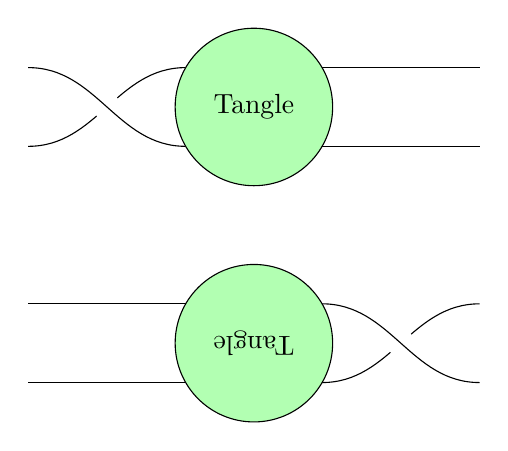
\begin{tikzpicture}
    \draw (0,0) to[out=0, in=180] (2, 1);
    \fill[white] (1, 0.5) circle (5pt);
    \draw (0,1) to[out=0, in=180] (2, 0);
    \filldraw[fill=green!30] ({2+sqrt(1-0.25)}, 0.5) circle (1);
    \draw ({2+2*sqrt(1-0.25)}, 1)--({4+2*sqrt(0.75)}, 1);
    \draw ({2+2*sqrt(1-0.25)}, 0)--({4+2*sqrt(0.75)}, 0);
    \node at ({2+sqrt(0.75)}, 0.5) {Tangle};

    \begin{scope}[shift={ ({4+2*sqrt(0.75)}, -2) }, rotate=180]
      \draw (0,0) to[out=0, in=180] (2, 1);
      \fill[white] (1, 0.5) circle (5pt);
      \draw (0,1) to[out=0, in=180] (2, 0);
      \filldraw[fill=green!30] ({2+sqrt(1-0.25)}, 0.5) circle (1);
      \draw ({2+2*sqrt(1-0.25)}, 1)--({4+2*sqrt(0.75)}, 1);
      \draw ({2+2*sqrt(1-0.25)}, 0)--({4+2*sqrt(0.75)}, 0);
      \node[rotate=180] at ({2+sqrt(0.75)}, 0.5) {Tangle};
    \end{scope}
  \end{tikzpicture}
  \caption{\label{flype}Wywracanie skarpety na lewą stronę, czyli \emph{flype}.}
\end{figure}

Słowo \emph{flype} pochodzi ze szkockiego i oznacza wywracanie skarpetki na lewą stronę. Chodzi o obracanie kołtuna (ang. \emph{tangle}) o 180 stopni (patrz. \cref{flype} lub \href{https://en.wikipedia.org/wiki/Flype}{wikipedia <3}). Kołtun to włożenie $n$ łuczków w $S^3$ tak, że ich $2n$ końców jest przyklejonych do $2n$ punktów zaznaczonych na granicy $S^3$.

\subsection{Linki rozszczepione (ang. \emph{split}) i pierwsze}

Definicja bycia alternującym linkiem jest analogiczna jak bycia alternującym węzłem, więc ją pominiemy. Zaczniemy od przymiotnika, który dotyczy tylko linków i nie ma łatwo osiągalnego tłumaczenia na język polski. To znaczy zastanowimy się, co to znaczy móc rozdzielić (rozszczepić) link $L$.

\begin{deff}[link i diagram rozszczepiony]
  Powiemy, że \buff{link $L$} (o co najmniej dwóch komponentach) zanurzony w $S^3$ jest \buff{rozszczepiony}, jeśli możemy $S^3$ podzielić na dwie kule $S^2$ tak, że każda ma po przynajmniej jednym komponencie $L$. 

  Definicja ta przenosi się na diagram $D\in S^2$ poprzez spłaszczenie tych sfer $S^2$ do zamkniętych krzywych. To znaczy, \buff{diagram $D$ jest rozszczepiony}, jeśli istnieje prosta krzywa zamknięta w $S^2\setminus D$, która dzieli je na dwa rozłączne dyski, każdy zawierający przynajmniej jeden komponent $D$.
\end{deff}

Link trywialny, czyli $O\;O$, jest w oczywisty sposób rozszczepialny.

\begin{thm}
  Link $L$ o alternującym diagramie $D$ jest rozszczepialny $\iff$ $D$ jest rozszczepialnym diagramem.
\end{thm}

{\color{red}
Dowód tego twierdzenia zostanie podany na koniec sekcji.
}

Na pierwszych zajęciach dowiedzieliśmy się, że nietrywialny węzeł $K$ jest pierwszy (ang. \emph{prime}), jeśli nie jest sumą spójną dwóch nietrywialnych węzłów. Moglibyśmy powiedzieć, że każda kula $S^2\subseteq S^3\setminus K$ przecinająca węzeł $K$ w dwóch punktach dzieli $S^3$ na dwa fragmenty, z czego jeden posiada "trywialny łuczek", tj. łuczek który bez problemu możemy rozsupłać przy pomocy ruchów Reidenmeistera. W podobny sposób możemy przenieść definicję pierwszości na linki i ich diagramy.

\begin{deff}[link i diagram pierwszy]
  \buff{Link $L\subseteq S^3$}, różny od linku (i węzła) trywialnego, jest \buff{pierwszy}, jeśli każda sfera $S^2$ przecinająca go w dwóch punktach dzieli $S^3$ na dwa fragmenty, z których jeden zawiera jeden trywialny łuczek $L$.

  \buff{Diagram $D\subseteq S^2$ jest pierwszy}, jeśli każda prosta krzywa zamknięta w $S^2$ przecinająca $D$ w dwóch punktach zawiera w swoim wnętrzu lub na zewnątrz diagram odpowiadający rozwiązywalnemu łuczkowi. Takie $D$ jest \acc{silnie pierwszy}, jeśli zawsze po takim rozcięciu znajdziemy diagram z zerową liczbą skrzyżowań. 
\end{deff}

Tutaj warto zauważyć, że jedynym linkiem, który jest jednocześnie pierwszy i rozszczepiony jest link trywialny $O\;O$.

Kolejne twierdzenie, na którego dowód musimy troszkę poczekać, które pozwala nam badać pierwszość linków alternujących przez pryzmat ich diagramów.
\begin{thm}
  Załóżmy, że $L$ jest linkiem o alternującym diagramie $D$. Wtedy $L$ jest linkiem pierwszym $\iff$ $D$ jest diagramem pierwszym.
\end{thm}

{\large\color{red}WRÓCIĆ TUTAJ, BO MI SIĘ CHWILOWO NIE CHCE}

\subsection{Po co nam to wszystko? Czyli o jeżach (między innymi)}

Zacznijmy od szybkiej informacji co to znaczy być powierzchnią. Oczywiście mówiąc powierzchnia mamy na myśli $2$-rozmaitość, czyli przestrzeń której każdy punkt ma otoczenie homeomorficzne z otwartym podzbiorem $\R^2$. Zamkniętych powierzchni nie ma bardzo dużo i każda taka powierzchnia jest wymieniona niżej
\begin{enumerate}
  \item sfera $S^2$
  \item suma spójna $n$ torusów $\mathbb{T}^2$
  \item suma spójna $n$ płaszczyzn rzutowych $\R P^2$
\end{enumerate}
Poza tym jest m.in. butelka Kleina (nieorientowalna, bez brzegu) czy wstęga M\"obiusa (nieorientowalna, z brzegiem).

Powiemy teraz, co to znaczy, że powierzchnia $F\subseteq M$, gdzie $M$ jest $3$-rozmaitością, jest niekompresowalna. Przy okazji dowiemy się, co to znaczy być dyskiem rozpinającym powierzchnię.

\begin{deff}[powierzchnia niekompresowalna] 
  Niech $F$ będzie powierzchnią różną od $S^2$ zanurzoną w $3$-rozmaitość $M$. Powiemy, że $F$ jest \buff{niekompresowalna}, jeśli każdy dysk $\Delta\subseteq M$ taki, że $\Delta\cap F=\partial\Delta$ (tzn. $\Delta$ \acc{rozpina} powierzchnię $F$) ogranicza dysk w $F$ (patrz \cref{pierwszy}).

  Sfera $S^2$ jest niekompresowalna, jeśli nie ogranicza $D^3$ w $M$.
\end{deff}

\begin{figure}%
\centering
\subfloat[][powierzchnia niekompresowalna]{ 
  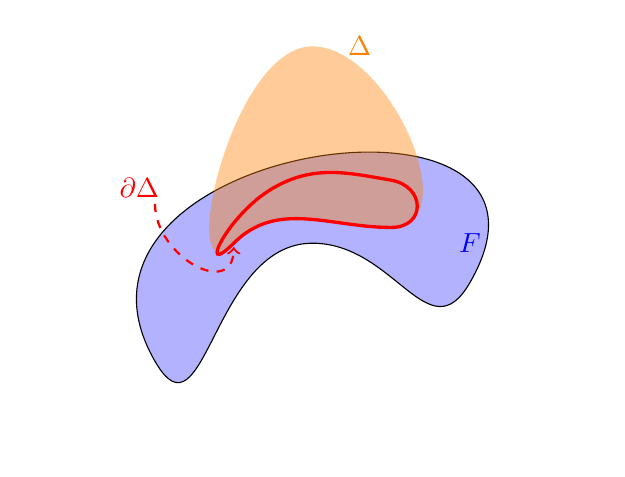
\begin{tikzpicture}
    \coordinate (a1) at (0,0);
    \coordinate (a2) at (-4, -1);
    \coordinate (a3) at (-2, 0.5);

    %\foreach \i in {1,...,3} \fill (a\i) circle (4pt);

    \filldraw[fill=blue!30] (a1) to[out=60, in=120, looseness=2] 
      (a2) to[out=-60, in=180, looseness=1.3] 
      (a3) to[out=0, in=-120, looseness=1.3] 
      (a1);
    \fill[opacity=0.4, orange] (-3, 0.5)to[out=45, in=180] (-1, 0.7) to[out=0, in=0] (-2, 3) to[out=180, in=180+45] (-3, 0.5);
    \draw[red, very thick] (-3, 0.5) to[out=45, in=180] (-1, 0.7) to[out=0, in=-10, looseness=1.9] (-1, 1.3) to[out=170, in=30, looseness=1] (-2.5, 1.2) to[out=210, in=180+45, looseness=2] (-3, 0.5);
    \draw[dashed, red, thick, ->] (-4, 1) to[out=-90, in=-90, looseness=1.5] (-3, 0.45);
    \node at (-4.2, 1.2) {$\color{red}\partial\Delta$};

    \node at (-1.4, 3) {$\color{orange}\Delta$};
    \node at (0, 0.5) {$\color{blue}F$};
  \end{tikzpicture}
}%
\qquad
\subfloat[][powierzchnia kompresowalna] {
  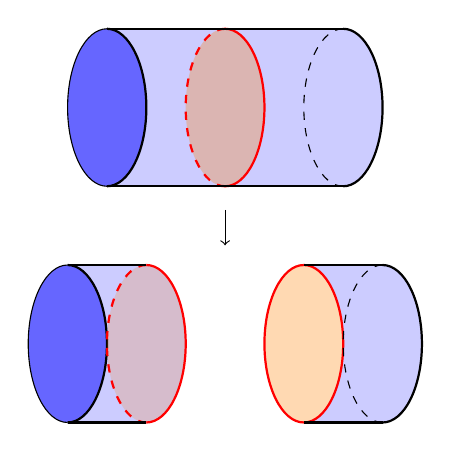
\begin{tikzpicture}
    \fill[blue!20] (0,0) rectangle (3, 2);
    \fill [blue!20] (3, 1) ellipse (0.5 and 1);
    \fill[blue!60] (0, 1) ellipse (0.5 and 1);

    \draw[thick] (0,0) arc (-90:90:0.5 and 1);
    \draw (0,0) arc (-90:-270:0.5 and 1);
    
    \fill[orange, opacity=0.3] (1.5, 1) ellipse (.5 and 1);
    \draw[thick, red] (1.5, 0) arc (-90:90:0.5 and 1);
    \draw[dashed, thick, red] (1.5,0) arc (-90:-270:0.5 and 1);
    
    \draw[thick] (3,0) arc (-90:90:0.5 and 1);
    \draw[dashed] (3,0) arc (-90:-270:0.5 and 1);
    \draw[thick] (0, 2)--(3, 2);
    \draw[thick] (0,0)--(3,0);

    \draw[->] (1.5, -0.3)--(1.5, -0.75);

    \begin{scope}[shift={(0, -3)}]
      \begin{scope}[shift={(-0.5, 0)}]
    \fill[blue!20] (0,0) rectangle (1, 2);
    \fill [blue!20] (1, 1) ellipse (0.5 and 1);
    \fill[blue!60] (0, 1) ellipse (0.5 and 1);

    \draw[thick] (0,0) arc (-90:90:0.5 and 1);
    \draw (0,0) arc (-90:-270:0.5 and 1);
    
    \fill[orange, opacity=0.2] (1, 1) ellipse (.5 and 1);
    \draw[thick, red] (1, 0) arc (-90:90:0.5 and 1);
    \draw[dashed, thick, red] (1,0) arc (-90:-270:0.5 and 1);
    
    % \draw[thick] (1,0) arc (-90:90:0.5 and 1);
    % \draw[dashed] (1,0) arc (-90:-270:0.5 and 1);
    \draw[thick] (0, 2)--(1, 2);
    \draw[thick] (0,0)--(1,0);
  \end{scope}


    \begin{scope}[shift={(0.5, 0)}]
    \fill[blue!20] (2,0) rectangle (3, 2);
    \fill [blue!20] (3, 1) ellipse (0.5 and 1);

    %\draw[thick] (0,0) arc (-90:90:0.5 and 1);
    %\draw (0,0) arc (-90:-270:0.5 and 1);
    
    \fill[orange!30] (2, 1) ellipse (.5 and 1);
    \draw[thick, red] (2, 0) arc (-90:90:0.5 and 1);
    \draw[thick, red] (2,0) arc (-90:-270:0.5 and 1);
    
    \draw[thick] (3,0) arc (-90:90:0.5 and 1);
    \draw[dashed] (3,0) arc (-90:-270:0.5 and 1);
    \draw[thick] (2, 2)--(3, 2);
    \draw[thick] (2,0)--(3,0);
  \end{scope}
  \end{scope}

  \end{tikzpicture}
}
\caption{\label{pierwszy} Powierzchnię (b) możemy rozciąć wzdłuż $\partial\Delta$ i zakleić dwoma kopiami $\Delta$, by dostać dwie "zakrętki". Jest tak, ponieważ otoczenie tubularne $\Delta$ ma ciekawy przekrój z $F$. W przypadku powierzchni (a) otoczenie tubularne $\Delta$ daje po prostu annulus na $F$. }%
\end{figure}

\begin{fuck}
  Niech $L$ będzie nierozszczepialnym, pierwszym i alternującym linkiem, a $F$ niech będzie zamkniętą niekompresowalną powierzchnią w $S^3\setminus L$. Wówczas istnieje dysk $\Delta$ rozpinający $F$ w $S^3$, który przecina $L$ w dokładnie jednym punkcie.
\end{fuck}

Żeby to zobaczyć, trzeba wyobrazić sobie \acc{najeżenie węzła/linku $L$}, czyli jego otoczenie tubularne (zamiast nitki mamy sznurek bawełniany o średnicy $5$mm). Takich otoczeń mamy dużo, dla każdego $\varepsilon>0$. Możemy więc wybierać otoczenia $U_n$ o średnicy $\frac{1}{n}$. Kiedy wyjmujemy z $S^3$ węzeł $K$ duża część $U_n$ zostaje, więc możemy wybierać duszczki $\Delta_n$, które mają przekrój z otoczneiem $U_n$ o średnicy $\frac{1}{n}$ na wysokości tylko jednego segmentu. Granica tych dyszczków nie jest już w $S^3\setminus L$, bo zahacza o otoczenie średnicy $0$, tzn. przecina się z węzłem $L$ w jednym punkcie.

\begin{fuck}
  Niech $L$ będzie nierozszczepialnym, pierwszym i alternującym linkiem. Każdy niekompresowalny torus $T$ zawarty w $S^3\setminus L$ jest równoległy do granicy najeżenia pewnego komponentu $L$.
\end{fuck}

\end{document}
